\section{Modelo Relacional}
\subsection{Imagem do Modelo Relacional}

\begin{figure}[H]
    \centering
    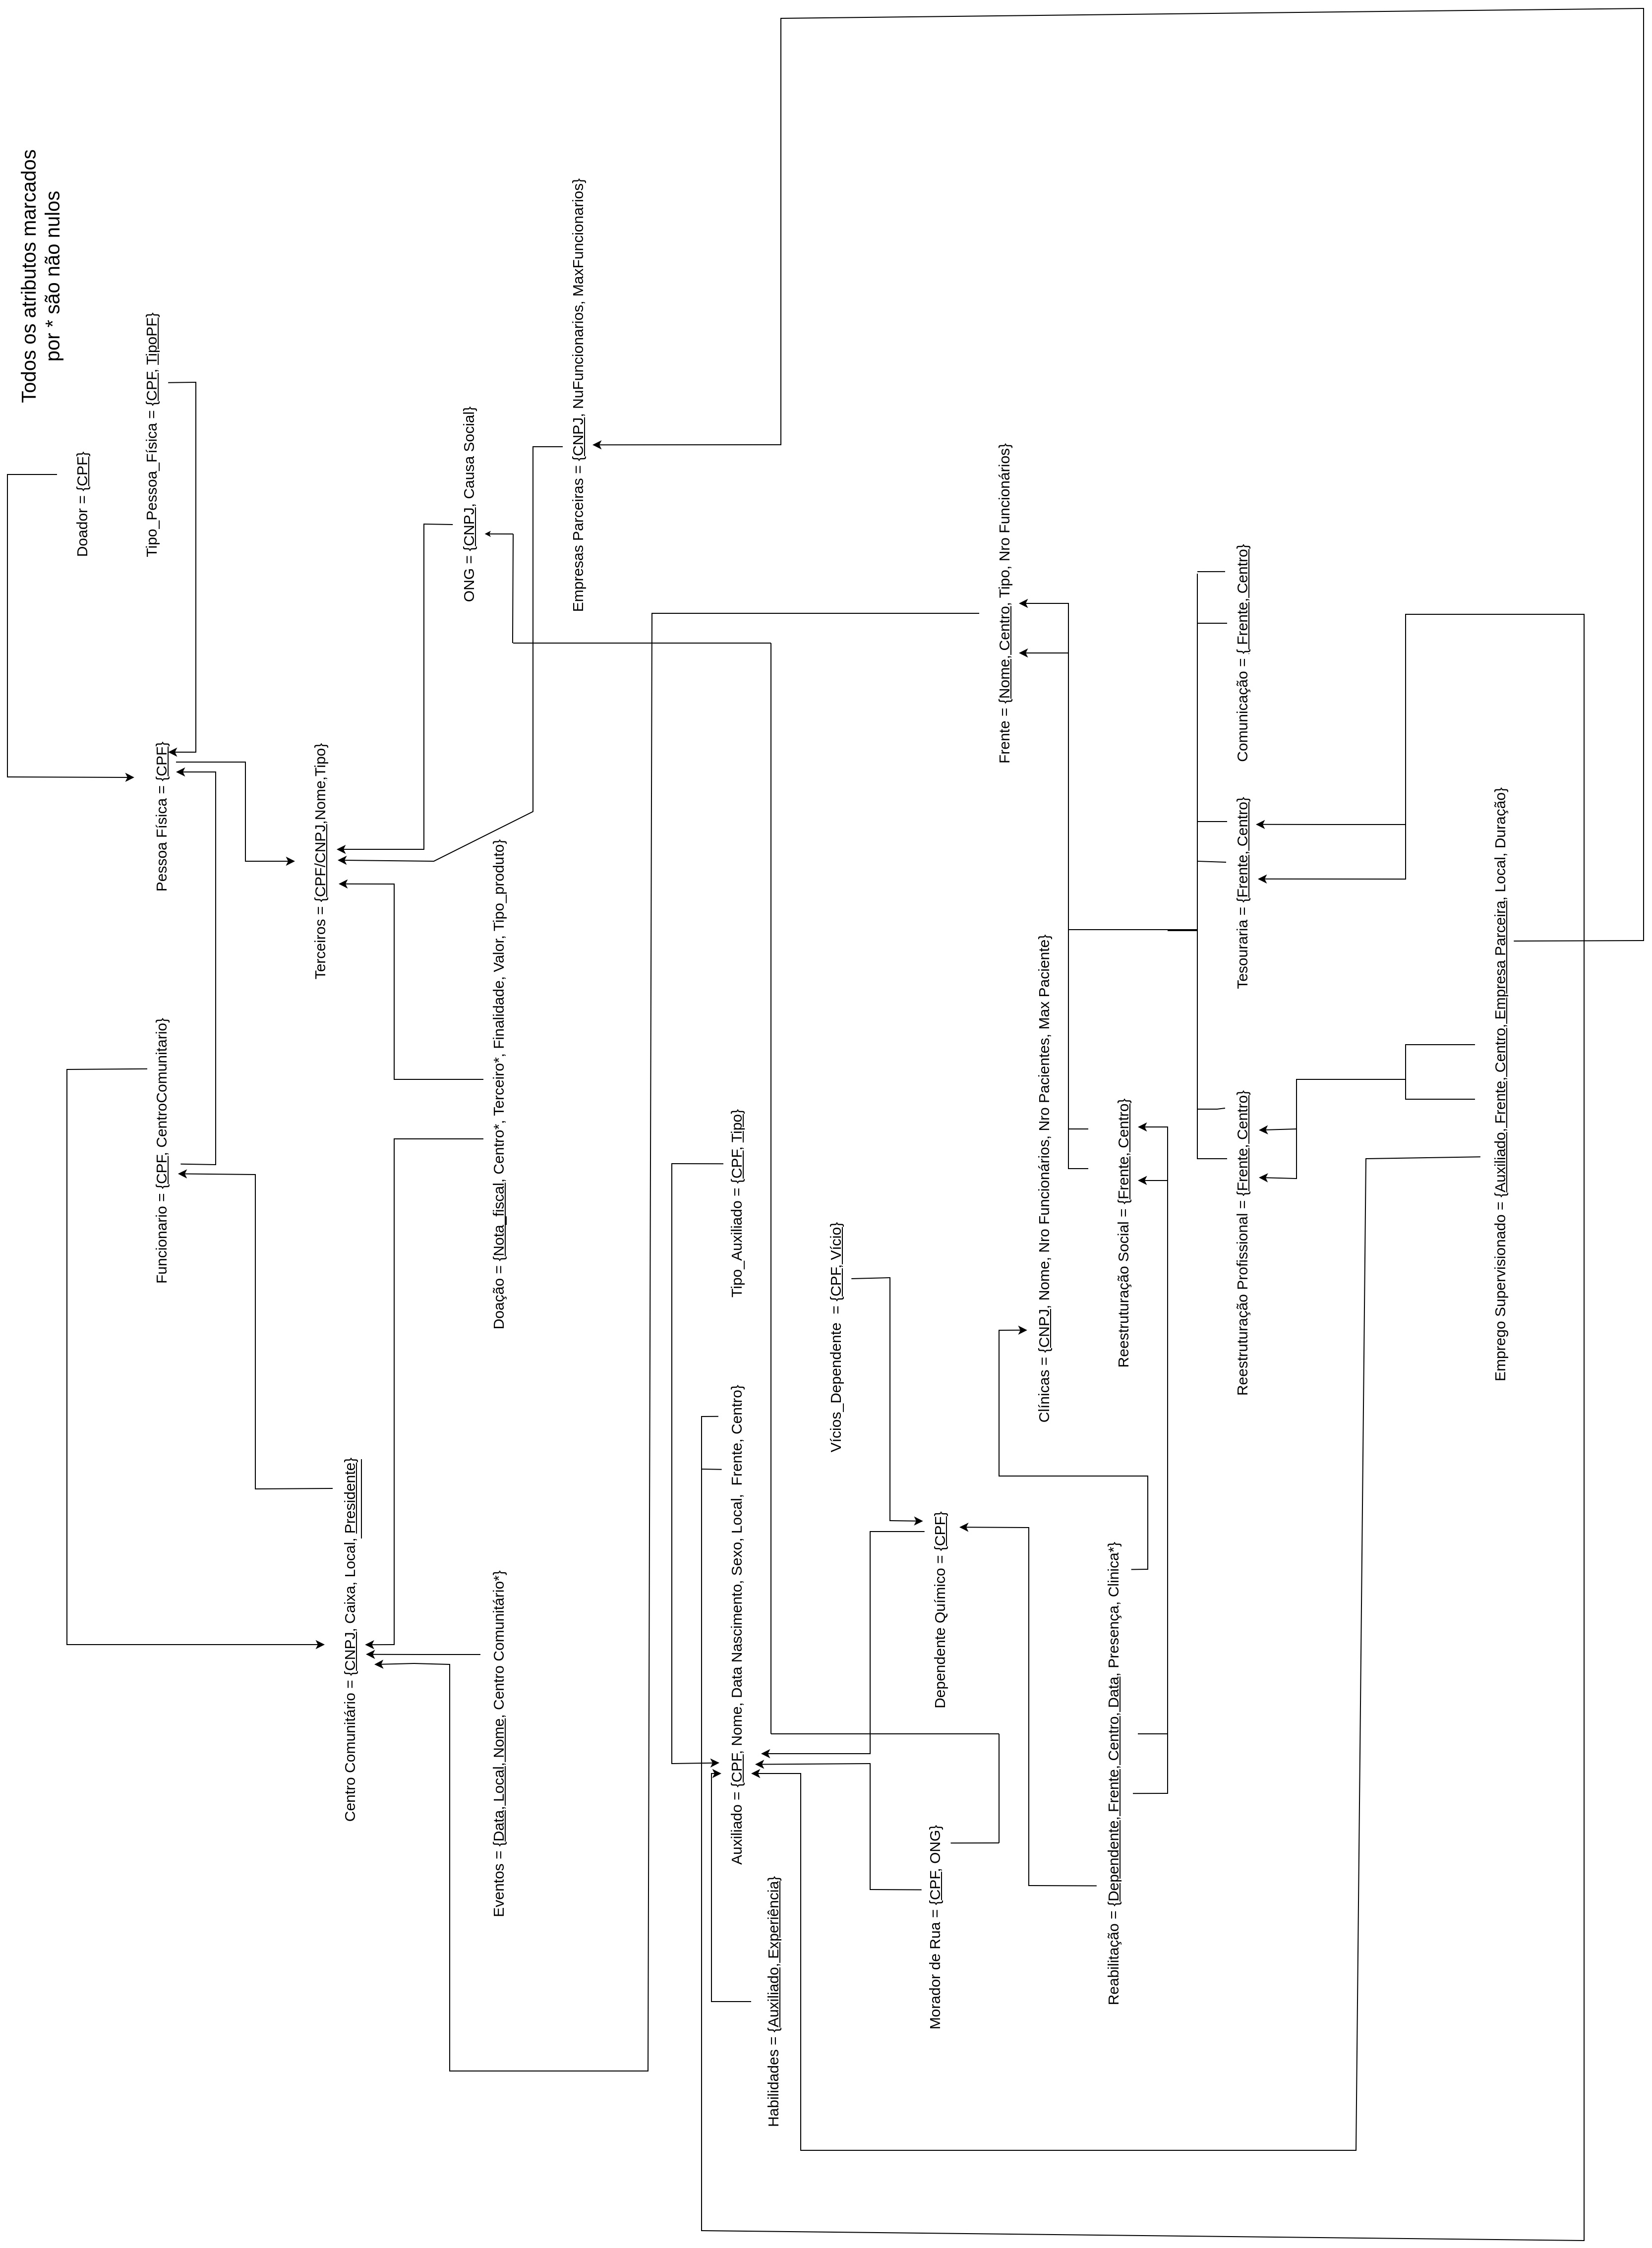
\includegraphics[scale=0.13]{images/Modelo_Relacional_VF.png}
    \label{fig:Relacional}
\end{figure}

\subsection{Restrições de integridade}
\begin{enumerate}
    \item \textbf{Possível inconsistência nas especializações totais (Doação, auxiliado)}
    
    A modelagem utilizada não garante uma especialização total dessas partes, sendo necessária atenção especial no processo de implementação.
    \item \textbf{Possível inconsistência na chave de terceiro}
    
    Como supracitado, a chave necessita ser CPF para Pessoas físicas e CNPJ para ONGS/Empresas parceiras. Nesse ponto, o tratamento ficará a cargo da implementação, sendo sugerida a utilização de RegEx em parceria com regras de entrada para garantir a funcionalidade.
    \item \textbf{Ciclo Presidente} $\xrightarrow[]{}$ \textbf{Centro comunitário}
    
    O entendimento correto desse ciclo demonstra que o Presidente de um centro comunitário deve ser um funcionário participante do mesmo.
\end{enumerate}

\subsection{Justificativas para a modelagem}
A seguir estão listadas as justificativas tomadas para a criação do modelo
relacional utilizando o modelo entidade relacionamento desenvolvido no tópico
anterior.

\begin{enumerate}

    \item \textbf{Modelagem 1:1 (Preside)}
    \\
    \textbf{Solução Adotada}: Devido a participação total, a melhor alternativa encontrada foi referenciar, dentro de centro comunitário, um presidente através de uma chave estrangeira com a presença do indicador de not null.
    \\
    \textbf{Desvantagens}: À priori, essa maneira é a ideal de representar a relação, não possuindo desvantagens evidentes.
    \\
    \textbf{Solução Alternativa}: Poderia-se criar uma tabela à parte, com tupla de centro e funcionário. Sendo centro chave primária e presidente chave secundária não nula, o efeito final seria semelhamte, mas haveria maior processamento.

    
    \item \textbf{Modelagem 1:N}
    \\
    \textbf{Solução Adotada}: Nestes casos, opta-se por modelar normalmente a entidade com cardinalidade "1" e inseri-la dentro da entidade com cardinalidade N. Em casos onde há participação total, essa inserção é acompanhada de um not null.
    \\
    \textbf{Vantagem}: Em relacionamentos com participação total, essa solução garante que esse campo nunca será nulo na hora de inserção em tabela.
    \\
    \textbf{Desvantagem}: Em situações como a relação de alojamento ou subsidia, onde não há participação total, a entidade que engloba a outra poderá conter campos vazios. Por se tratar de pouca informação, não é um empecilho realmente grande.
    \\
    \textbf{Solução Alternativa}: Poderia-se criar uma nova tabela referenciando por chave estrangeira cada uma das entidades. Contudo, trata-se de uma ação muito exagerada - devido a criação de tabela, indexação de valores - para reduzir um problema que à priori é muito pouco impactante (na parte relativa ao "Aloja"), por essa razão, opta-se pela abordagem realizada.

    \item \textbf{Mapeamento da agregação Reabilitação}
    \\
    \textbf{Solução Adotada}: Criação de uma tabela contendo as chaves da clínica, frente (que no caso, herda a também a chave de Centro, por ser entidade fraca) e do dependente químico.
    \\
    \textbf{Vantagem}: Permite a modelagem e unicidade dos tratamentos de forma idealizada, permitindo manter um controle da presença.
    \\ 
    \textbf{Desvantagens}: Como possui uma entidade fraca, o resultado final é muito sujo, por possuir muitas chaves estrangeiras.
    \\
    \textbf{Solução alternativa}: A modelagem poderia possuir um ID, reduzindo esses custos. Contudo, a presença das chaves estrangeiras torna mais semântico o entendimento da agregação e não é um impacto realmente grande a ponto de necessitar de uma troca.

    \item \textbf{Mapeamento da agregação Emprego Supervisionado }
    \\
    \textbf{Solução Adotada}: Criação de uma tabela contendo as chaves da empresa, frente (que no caso, herda a também a chave de Centro, por ser entidade fraca) e do auxiliado.
    \\
    \textbf{Vantagem}: Permite a modelagem e unicidade dos tratamentos de forma idealizada, permitindo manter um controle da atuação do auxiliado.
    \\ 
    \textbf{Desvantagens}: Como possui uma entidade fraca, o resultado final é muito sujo, por possuir muitas chaves estrangeiras.
    \\
    \textbf{Solução alternativa}: A modelagem poderia possuir um ID, reduzindo esses custos. Contudo, a presença das chaves estrangeiras torna mais semântico o entendimento da agregação e não é um impacto realmente grande a ponto de necessitar de uma troca.

    \item Mapeamento da agregação Doação
    \\
    \textbf{Solução Adotada}: Criação de uma tabela com chave primária sendo nota fiscal. Há também a referência tanto ao Centro como ao terceiro, mas à parte da chave principal.
    \\
    \textbf{Vantagem}: A utilização de uma nota fiscal aumenta a eficiência do sistema e, desta maneira, a agregação criada permite o controle de forma rápida e direcionada das doações recebidas pelo centro.
    \\ 
    \textbf{Desvantagens}: Não há.

    \textbf{Solução Alternativa}: O conjunto poderia ser identificado pelo doador, centro comunitário e data/hora, por exemplo. Contudo, a pesquisa ficaria mais lenta e não há realmente uma razão para realizar a troca de nota fiscal.

    \item \textbf{Mapeamento especialização Terceiros, Frente}:
    \\
    \textbf{Solução Adotada}: Criação de uma tabela geral, contendo a chave primária e atributos gerais. Criação de uma tabela específica, contendo os atributos específicos e, por fim, criação de uma tabela de controle, herdando a chave da entidade geral para tentar garantir seu disjoint.
    \\
    \textbf{Vantagem}: Por conta das entidades específicas possuírem relações próprias, faz-se necessário sua modelagem. A criação de uma tabela de controle facilita a busca e torna o projeto mais eficiente

    \textbf{Desvantagens}: As entidades específicas possuem poucos ou nenhum atributo próprio, tornando um pouco desperdício sua modelagem à parte. Todas elas são bem semelhantes em seus dados, podendo haver também uma repetição muito grande. Em alguns casos, com um erro por parte da inserção bem exagerado, poderia-se criar uma situação onde o Disjoint não fosse garantido. 

    \textbf{Soluções Alternativas}: A modelagem podia consistir de uma criação apenas das entidades específicas, sem a criação de uma geral. Contudo, haveria muita repetição de relacionamentos, uma vez que cada uma deveria replicar as relações da entidade geral retirada.

     \item \textbf{Mapeamento especialização Auxiliado}:
    \\
    \textbf{Solução Adotada}: Criação de uma tabela geral, contendo a chave primária e atributos gerais, bem como o atributo de especialização. Criação de uma tabela específica, contendo os atributos específicos.
    \\
    \textbf{Vantagem}: Por conta das entidades específicas possuírem relações próprias, faz-se necessário sua modelagem. Evita a criação de uma tabela extra de controle

    \textbf{Desvantagens}: As buscas podem se tornar um pouco lentas, por não se ter uma correlação direta entre Auxiliado e Tipo, como anteriormente usado na tabela de controle. Em discussão com o grupo, concluímos que essa maneira era mais limpa e valeria a pena mesmo assim. Não garante também a especialização total. 

    \textbf{Soluções Alternativas}: A modelagem poderia seguir os padrões anteriores, utilizando uma tabela de controle. No fim, a indexação talvez não fizesse valer a pena, haja vista que essa consulta além de não ser tão utilizada, não fica lenta o suficiente na modelagem usada para ser necessário sua mudança.
    
    
    \item \textbf{Mapeamento da especialização Doação}
    \\
    \textbf{Solução Adotada}: Unificação de todos os atributos das entidades específicas na tabela única doação.
    \\
    \textbf{Vantagem}: A utilização de menos tabelas faz com que o tempo de busca seja favorecido, pois não será necessário acessar duas tabelas distintas e é diminuído o tamanho em armazenamento da base de dados.
    \\ 
    \textbf{Desvantagens}: Pode gerar muitos valores nulos caso várias doações de apenas um tipo, monetária ou de produto, sejam realizadas.

    \textbf{Solução Alternativa}: Construir uma tabela para cada entidade específica, possuindo uma chave estrangeira como chave principal, a qual seria o número de nota fiscal da doação referente, além de uma tabela para categorizar os tipos, também tendo o número da nota fiscal como chave estrangeira e chave primária da tabela, que é composta com tipo.

    \item \textbf{Mapeamento da especialização Pessoa Física}
    \\
    \textbf{Solução Adotada}: Criação de uma tabela geral, contendo a chave primária e atributos gerais, bem como o atributo de especialização. Criação de uma tabela específica, contendo os atributos específicos. 
    \\
    \textbf{Vantagem}: Por conta das entidades específicas possuírem relações próprias, faz-se necessário sua modelagem. Evita a criação de uma tabela extra de controle, melhorando o tempo no quesito de indexação.

    \textbf{Desvantagens}: As buscas podem se tornar um pouco lentas, por não se ter uma correlação direta entre Pessoa Física e Tipo, como anteriormente usado na tabela de controle. Por não ser necessário especialização total, é uma boa abordagem.

    \textbf{Soluções Alternativas}: A modelagem poderia seguir os padrões anteriores, utilizando uma tabela de controle. No fim, a indexação talvez não fizesse valer a pena, haja vista que essa consulta além de não ser tão utilizada, não fica lenta o suficiente na modelagem usada para ser necessário sua mudança.
    
    \item \textbf{Atributos Multivalorados (Vícios, Habilidades)}:
    \textbf{Solução Adotada}: Seguiu-se a modelagem padrão para atributos multivalorados, onde cria-se uma tabela, herdando a chave principal de sua entidade-mãe que fará parte da chave primária da próxima tabela, juntamente com o seu diferenciador. Por exemplo, para a tabela de vícios, as chaves serão compostas pelo CPF do auxiliado, bem como pelo vício em si. De forma análoga para as habilidades, onde a tabela de habilidades possuirá o CPF do indivíduo e, para cada habilidade, será gerada uma nova tupla.
    \\
    \textbf{Vantagem}: A modelagem facilita a correlação dos valores, sendo amplamente utilizada para essas situações.

    \textbf{Desvantagens}: Pode-se ter valores nulos e o processo de indexação em si consome processamento.

    \textbf{Soluções Alternativas}: Dependendo da importância dada à estes pontos, como trata-se de atributos multivalorados, caso eles sejam considerados descartáveis, poderiam ser apresentados como uma grande string univalorada. Futuramente, em tratamento de aplicação, através de um parser, esses valores poderiam ser retornados.
    
    
    \item \textbf{Mapeamento do atributo derivado `idade` da entidade `Auxiliado`}
    
    \textbf{Solução adotada:} O atributo `idade` da entidade `Auxiliado` foi mapeado como sendo derivado por seu baixo custo de calculo e para evitar colocar informações redundantes no modelo. Portanto, como foi considerado atributo derivado ele não foi colocado na tabela `auxiliado` no modelo relacional.
    \\
    \textbf{Vantagens: } Diminui a quantidade de dados armazenados nesta entidade. 
    \\
    \textbf{Desvantagens: } O cálculo que é necessário para ter a informação do atributo, desacelera possíveis tratamentos.
    \\
    \textbf{Soluções Alternativas: } Colocar o atributo não sendo derivado. Isso implicaria que todos os dias um cálculo deverá ser feito para todas os membros daquela entidade, o que pode ser custoso de acordo com o tamanho da entidade.
    
\end{enumerate}